\section{Ngữ cảnh bài toán}
    \subsection{Mô tả chung}
        \quad Quản lý rác thải đô thị là một trong những vấn đề quan trọng mà nhiều nước hiện nay đang phải đối mặt và được xem là một trong những tiêu chí quan trọng trong mục tiêu phát triển bền vững (Sustainable Development Goals). Khi mà các nước đang phát triển ưu tiên phát triển công nghiệp hóa hiện đại hóa thì việc xử lý rác thải khó phân hủy vẫn còn đang vận hành một cách kém hiệu quả.\\
        
        \begin{figure}[h]
            \centering
            
\includegraphics[width=1\linewidth]{imgs/SDG.jpg}
            \caption{Sustainable Development Goals}
        \end{figure}
        
        \quad Mục tiêu của bài tập lớn lần này là tạo ra một hệ thống giúp quản lý việc thu thập rác thải, từ đó đưa đến những tác động tích cực lên thành phố, xã hội và môi trường.
    \subsection{Khảo sát thực tế}
        \quad Mạng lưới thu gom, vận chuyển rác thải sinh hoạt từ các điểm hẹn về trạm trung chuyển và vận chuyển đến các khu liên hợp xử lý trên địa bàn TP do ba đơn vị cùng thực hiện. Đó là Công ty TNHH MTV Môi trường đô thị TP.HCM (CITENCO), Công ty TNHH MTV Dịch vụ công ích quận, huyện và Hợp tác xã (HTX) Vận tải công nông. \\
        \quad Để vận hành hệ thống thu gom, vận chuyển rác thải sinh hoạt, hiện nay TP có khoảng 908 điểm hẹn tập trung rác (cả nội thành và ngoại thành) trong đó giả định rằng thành phố Thủ Đức có 227 điểm (chiếm 25\%). CITENCO là một công ty có nhiều năm kinh nghiệm hoạt động trong lĩnh vực thu gom, vận chuyển chất thải, dưới đây là danh sách một số phương tiện vận chuyển của họ (Lưu ý là không phải phương tiện nào cũng cần dùng, nên dùng tối giản nhất có thể theo yêu cầu của bài toán).
        
        \begin{tblr}{
            width=1\linewidth,
            hlines,
            vlines,
            colspec={X[-2]X[2]X[3]X[2]X[5]},
            columns = {valign = m, },
            column{1} = {halign = c, },
            row{1} = {halign = c, valign = m, bg = lightgray, fg = black},
        }
            {\textbf{STT} & \textbf{Phương tiện} & \textbf{Trọng tải} & \textbf{Số lượng} & \textbf{Hoạt động} }  \\
            1 & Thùng rác & 240L, 660L & 630 & Thu gom rác sinh hoạt\\
            2 & Container & 12m3 - 18m3 & 101 & Lưu chứa, vận chuyển\\
            3 & Xuồng & 8,5m3 & 110 & Thu gom rác sinh hoạt\\
            4 & Xe ép nhỏ &         &    & \\
            &           & < 3 tấn & 44 & Thu gom rác sinh hoạt\\
            &           & 3 tấn - 7 tấn & 12 & Thu gom rác sinh hoạt\\
            &           & 7 tấn - 9 tấn & 12 & Thu gom, vận chuyển rác sinh hoạt\\
            5 & Xe ép lớn & > 9 tấn & 44 & Vận chuyển rác sinh hoạt\\
            6 & Xe tải Benz & 2,5 tấn & 7 & Vận chuyển rác sinh hoạt\\
            7 & Xe tải nhẹ & 4,5 tấn & 7 & Thu gom rác sinh hoạt\\
            8 & Xe tải cẩu & 1,9 - 13,5 tấn & 3 & Thu gom rác sinh hoạt\\
            9 & Xe tải lớn & 12 tấn & 9 & Thu gom rác sinh hoạt\\
            10 & Cẩu cạp & 2 tấn & 4 & Thu gom rác sinh hoạt \\
            11 & Xe Hooklift & > 9 tấn & 61 & Vận chuyển rác sinh hoạt, nước rỉ rác\\
        \end{tblr}
        
        \vspace{0.7cm}
        
        \quad Công ty CITENCO sẽ có một đội ngũ nhân viên bao gồm các janitors và collectors sẽ sử dụng các phương tiện như trên để thực hiện thu gom rác và các back officers với nhiệm vụ quản lý hệ thống, xếp lịch cho các janitors và collectors. Tại thành phố Thủ Đức hiện tại có 34 phường tương ứng với 34 điểm thu gom rác, dưới đây là bản đồ của 34 phường. (Lưu ý: Khu đô thị Đại học Quốc gia Thành phố Hồ Chí Minh có diện tích phần lớn trong địa phần phường Đông Hòa, thành phố Dĩ An, tỉnh Bình Dương nên giả định rằng thu gom rác khu vực này sẽ do thành phố Dĩ An quản lý).
        
        \quad Giả định vị trí của các điểm thu gom rác được đặt tại trung tâm mỗi phường của thành phố Thủ Đức, bao gồm:
        \begin{enumerate}
            \item Tân Phú: UBND phường Tân Phú.
            \item Long Bình: Ủy Ban Nhân Dân Phường Long Bình.
            \item Long Thạnh Mỹ: UBND Phường Long Thạnh Mỹ, Quận 9.
            \item Long Phước: UBND phường Long Phước.
            \item Trường Thạch: UBND phường Trường Thạch.
            \item Long Trường: UBND phường Long Trường.
            \item Phú Hữu: UBND phường Phú Hữu.
            \item Tăng Nhơn Phú B: UBND phường Tăng Nhơn Phú B.
            \item Tăng Nhơn Phú A: UBND phường Tăng Nhơn Phú A.
            \item Hiệp Phú: Ủy Ban Nhân Dân Phường Hiệp Phú.
            \item Phước Long B: UBND phường Phước Long B.
            \item Phước Long A: UBND phường Phước Long A.
            \item Phước Bình: UBND phường Phước Bình.
            \item Cát Lái: UBND phường Cát Lái.
            \item Bình Trưng Tây: UBND phường Bình Trưng Tây.
            \item Bình Trưng Đông: Ủy ban nhân dân phường Bình Trưng Đông.
            \item An Phú: UBND phường An Phú.
            \item Thạnh Mỹ Lợi: UBND phường Thạnh Mỹ Lợi. 
            \item Thảo Điền: UBND phường Thảo Điền.
            \item An Lợi Đông: UBND phường An Lợi Đông.
            \item An Khánh: UBND phường An Khánh.
            \item Thủ Thiêm: Tháp thông gió Hầm Thủ Thiêm.
            \item Trường Thọ: UBND phường Trường Thọ.
            \item Bình Thọ: UBND phường Bình Thọ.
            \item Linh Chiểu: UBND phường Linh Chiều.
            \item Linh Đông: UBND phường Linh Đông.
            \item Linh Tây: UBND phường Linh Tây.
            \item Linh Xuân: UBND phường Linh Xuân.
            \item Linh Trung: UBND phường Linh Trung.
            \item Tam Bình: UBND phường Tam Bình.
            \item Tam Phú: UBND phường Tam Phú.
            \item Bình Chiểu: UBND phường Bình Chiểu.
            \item Hiệp Bình Chánh: UBND phường Hiệp Bình Chánh.
            \item Hiệp Bình Phước: UBND phường Hiệp Bình Phước.
        \end{enumerate}
        
        \newpage
        \begin{figure}[h]
            \centering
            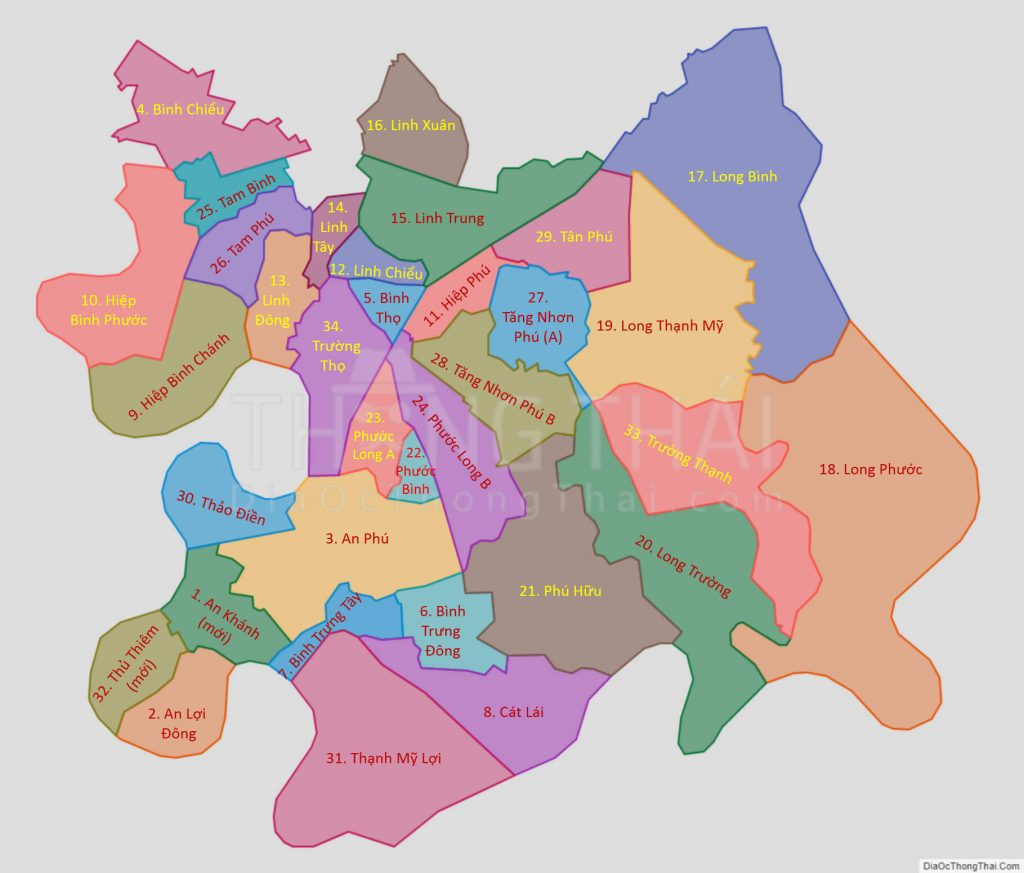
\includegraphics[width=1\linewidth]{imgs/map.jpg}
            \caption{Các phường trong thành phố Thủ Đức}
        \end{figure}
        
        \quad Tại mỗi điểm thu gom chất thải sẽ có các thùng phân loại rác thải, bao gồm rác thải hữu cơ, rác thải vô cơ, rác thải tái chế, rác thải không tái chế và rác thải không phân loại được.
        
        \quad Các phương tiện, thiết bị của CITENCO sẽ tập trung tại 3 địa điểm chính (Depot) tại quận 2 (cũ), quận 9 (cũ) và quận Thủ Đức (cũ):
        \begin{enumerate}
            \item Quận 2: Depot tại Cat Lai Port.
            \item Quận 9: Depot Tân Cảng Suối Tiên.
            \item Quận Thủ Đức: Depot tại Cảng Phúc Long.
        \end{enumerate}
        
        \quad Sau khi thu gom thì rác sẽ được đưa về 2 trạm trung chuyển của CITENCO đó là Trạm trung chuyển 691 Quang Trung, quận Gò Vấp và trạm trung chuyển số 01 Tống Văn Trân, quận 11. Sau đó sẽ được đưa về Khu liên hợp Xử lý Chất thải Đa Phước tại huyện Bình Chánh; Bãi chôn lấp Phước Hiệp tại huyện Củ Chi sẽ đóng vai trò dự phòng cho khu Đa Phước. 

        \quad Sau khi thực hiện khảo sát thực tế,nhóm nhận thấy tình hình thực tế không phù hợp với yêu cầu đặt ra của đề bài ban đàu, vì vậy nhóm chúng em xin được giả định bối cảnh của dự án như sau:
        
        \quad Một công ty xử lý rác thải bao gồm 3 loại nhân viên:
        \begin{itemize}
            \item Nhân viên giám sát (Back officer): Thực hiện nhiệm vụ giám sát và phân công lịch làm cho các công nhân.
            \item Nhân viên chở rác (Collector): Thực hiện việc lái xe rác và thu gom rác ở các điểm tập trung (MCPs).
            \item Nhân viên gom rác (Janitor): Thực hiện thu gom rác ở các hộ gia đình và đưa tới các điểm tập trung (MCPs).
        \end{itemize}
        
        \quad Lịch làm cũng như công việc trong ngày của công nhân được phân công bởi nhân viên giám sát, và sẽ được thay đổi theo tuần. Nhân viên giám sát đồng thời cũng quản lý việc phân công phương tiện và tuyến đường của chúng. Phương tiện và tuyến đường đi sẽ được thay đổi mỗi tháng một lần. Hằng ngày, nhân viên giám sát sẽ gửi thông tin về công việc trong ngày cho công nhân. Nhân viên thu gom rác sẽ tới từng nhà nhân thu gom rác vào các xe đẩy, sau đó đưa chúng tới điểm tập trung rác thải (MCPs), tại đây rác thải sẽ được các xe rác lớn do nhân viên chở rác lái thu gom và đưa đến nhà máy xử lý. Sau khi hoàn thành công việc, công nhân có thể xác nhận hoàn thành và tan ca.





